\documentclass[tikz,margin=1mm]{standalone}
\usepackage{tikz}
\usepackage{pgfplots}
\usepackage{physics,xfrac}

\pgfplotsset{compat=newest} %compat=1.10

\usepgfplotslibrary{fillbetween}
\usetikzlibrary{positioning,calc,decorations.markings}
% calc enables \foreach

\begin{document}

\newcommand\offset{1}
\newcommand\mycolor{black}

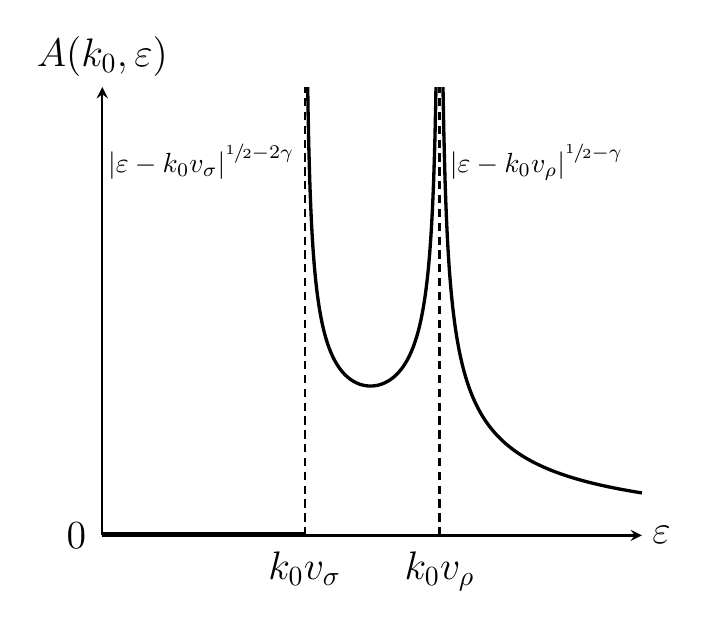
\begin{tikzpicture}
\begin{axis}[
    axis on top = false,
    thick,
    axis y line = left,
    axis x line = bottom,
    label style={font=\Large},
    tick label style={font=\Large},
    xtick style={draw=none},
    ytick style={draw=none},
    xticklabels={,,,$k_{0}v_{\sigma}$,$k_{0}v_{\rho}$},
    yticklabels={,0},
    xlabel = $\varepsilon$,
    xlabel     style={at={(1,0)},right},
    ylabel     style={at={(0,1)},above,rotate=-90},
    ylabel = {$A(k_{0},\varepsilon)$},
    xmin=7, xmax=15,
    ymin=0, ymax=3,
    % enlargelimits
]
    \pgfmathsetmacro{\Krho}{0.7};
    \pgfmathsetmacro{\Ksig}{0.8};
    \pgfmathsetmacro{\vrho}{1.2};
    \pgfmathsetmacro{\vsig}{1};
    \pgfmathsetmacro{\gmma}{(\Krho+1/\Krho-2)/8+(\Ksig+1/\Ksig-2)/8};
    \pgfmathsetmacro{\k}{10};
    
    \addplot[domain=\k*\vsig:20,samples=1000,very thick] {1/(abs(x-\vrho*\k)^(0.5-\gmma))/(abs(x-\vsig*\k)^(0.5-2*\gmma))};
    \draw[very thick] (0,0.01)--(\k*\vsig,0.01);
    
    \draw[densely dashed](10,0)--(10,5);
    \draw[densely dashed](12,0)--(12,5);
    
    \node[anchor=east]() at (\k*\vsig,2.5){$\abs{\varepsilon-k_{0}v_{\sigma}}^{\sfrac{1}{2}-2\gamma}$};
    \node[anchor=west]() at (\k*\vrho,2.5){$\abs{\varepsilon-k_{0}v_{\rho}}^{\sfrac{1}{2}-\gamma}$};
\end{axis}
\end{tikzpicture}
\end{document}